\chapter{System Architecture}
\label{chap:arch}

This chapter presents information concerning the architecture of the software
system both from the static and dynamic viewpoints. The static viewpoint focuses
on the physical architecture (hardware) required to deploy and run the
software system along with the manner in which the components that make such
software system are grouped. On the other hand, the dynamic viewpoint focuses on
the behaviour of the software system at runtime. 

The static information is presented through the \gls{Deployment View} and the
\gls{Implementation View}. The dynamic aspects of the system are presented by
means of the \gls{UI Processing View}.


\section{Deployment view}
System$'$s architecture follows client-server software
architecture with three layers.

\begin{figure}
\begin{center}
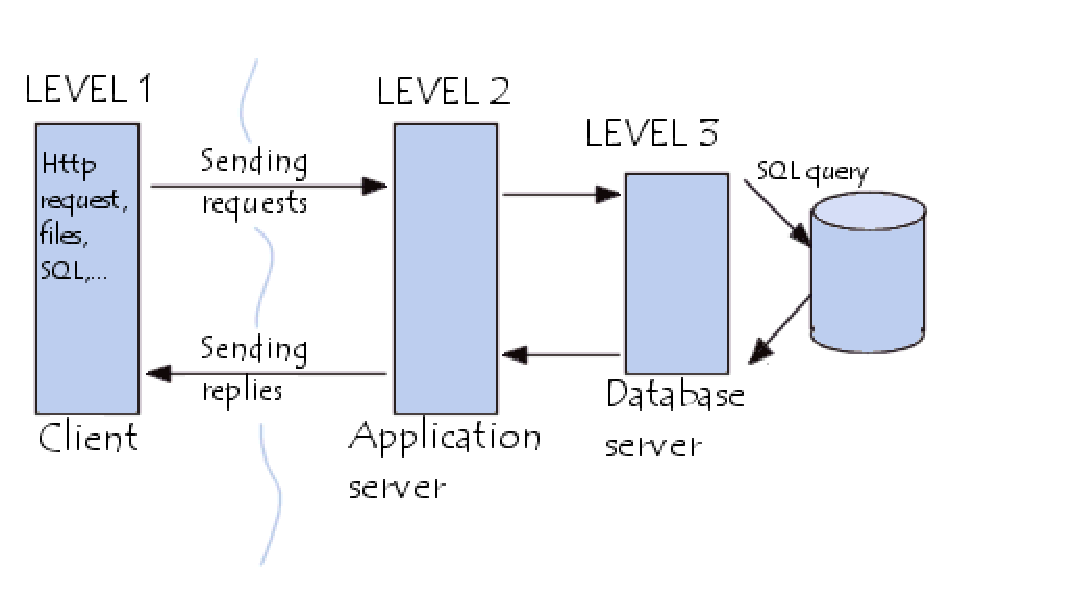
\includegraphics[width=\textwidth]{./images/c4deploymentview.eps}
\end{center}
\caption{Deployment View}
\label{fig:Deployment View}
\end{figure} 



\section{Implementation view}
The \gls{Implementation View} describes each software system component and how
they are organised and combined to make the targeted software system.




\subsection{Component xx.yy.zz.c1}
TODO

\subsection{Component xx.yy.zz.c2}
TODO

\subsection{Component xx.yy.zz.c3}
TODO





\section{UI Processing view}
A \gls{UI Processing View} is aimed at explaining the required message exchanges
to achieve the launching of a system operation (specified in the \msrmessir
Analysis Document). These required message exchanges (which are not specified in
the \msrmessir Analysis Document) make part of the user interface (UI). Thus, the
main interest of a UI Processing View is to describe the design choices made
at the UI level, such that a system operation is launched. The description
of a UI Processing View is given by means of a UML Sequence Diagram. 


A complete Design Document should contain a UI Processing View for each
non-proactive system operation specified in the \msrmessir Analysis Document, as
such kind of system operations are launched by actors through UIs that allows
them to make so. 



\subsection{UI Processing view for system operation oeSystemOperation1}
TODO

 
\subsection{UI Processing view for system operation oeSystemOperation2}
TODO


\subsection{UI Processing view for system operation oeSystemOperation3}
TODO





\section{Non-functional runtime concerns}
The description of the runtime processes should be complemented with free
textual information regarding concurrency, distribution, performance and scalability aspects.


\subsection{Performance}
TODO



\subsection{Concurrency and Parallelism}
TODO




\subsection{Scalability}
TODO






